\documentclass[twoside]{book}

% Packages required by doxygen
\usepackage{fixltx2e}
\usepackage{calc}
\usepackage{doxygen}
\usepackage[export]{adjustbox} % also loads graphicx
\usepackage{graphicx}
\usepackage[utf8]{inputenc}
\usepackage{makeidx}
\usepackage{multicol}
\usepackage{multirow}
\PassOptionsToPackage{warn}{textcomp}
\usepackage{textcomp}
\usepackage[nointegrals]{wasysym}
\usepackage[table]{xcolor}

% Font selection
\usepackage[T1]{fontenc}
\usepackage[scaled=.90]{helvet}
\usepackage{courier}
\usepackage{amssymb}
\usepackage{sectsty}
\renewcommand{\familydefault}{\sfdefault}
\allsectionsfont{%
  \fontseries{bc}\selectfont%
  \color{darkgray}%
}
\renewcommand{\DoxyLabelFont}{%
  \fontseries{bc}\selectfont%
  \color{darkgray}%
}
\newcommand{\+}{\discretionary{\mbox{\scriptsize$\hookleftarrow$}}{}{}}

% Page & text layout
\usepackage{geometry}
\geometry{%
  a4paper,%
  top=2.5cm,%
  bottom=2.5cm,%
  left=2.5cm,%
  right=2.5cm%
}
\tolerance=750
\hfuzz=15pt
\hbadness=750
\setlength{\emergencystretch}{15pt}
\setlength{\parindent}{0cm}
\setlength{\parskip}{3ex plus 2ex minus 2ex}
\makeatletter
\renewcommand{\paragraph}{%
  \@startsection{paragraph}{4}{0ex}{-1.0ex}{1.0ex}{%
    \normalfont\normalsize\bfseries\SS@parafont%
  }%
}
\renewcommand{\subparagraph}{%
  \@startsection{subparagraph}{5}{0ex}{-1.0ex}{1.0ex}{%
    \normalfont\normalsize\bfseries\SS@subparafont%
  }%
}
\makeatother

% Headers & footers
\usepackage{fancyhdr}
\pagestyle{fancyplain}
\fancyhead[LE]{\fancyplain{}{\bfseries\thepage}}
\fancyhead[CE]{\fancyplain{}{}}
\fancyhead[RE]{\fancyplain{}{\bfseries\leftmark}}
\fancyhead[LO]{\fancyplain{}{\bfseries\rightmark}}
\fancyhead[CO]{\fancyplain{}{}}
\fancyhead[RO]{\fancyplain{}{\bfseries\thepage}}
\fancyfoot[LE]{\fancyplain{}{}}
\fancyfoot[CE]{\fancyplain{}{}}
\fancyfoot[RE]{\fancyplain{}{\bfseries\scriptsize Generated by Doxygen }}
\fancyfoot[LO]{\fancyplain{}{\bfseries\scriptsize Generated by Doxygen }}
\fancyfoot[CO]{\fancyplain{}{}}
\fancyfoot[RO]{\fancyplain{}{}}
\renewcommand{\footrulewidth}{0.4pt}
\renewcommand{\chaptermark}[1]{%
  \markboth{#1}{}%
}
\renewcommand{\sectionmark}[1]{%
  \markright{\thesection\ #1}%
}

% Indices & bibliography
\usepackage{natbib}
\usepackage[titles]{tocloft}
\setcounter{tocdepth}{3}
\setcounter{secnumdepth}{5}
\makeindex

% Hyperlinks (required, but should be loaded last)
\usepackage{ifpdf}
\ifpdf
  \usepackage[pdftex,pagebackref=true]{hyperref}
\else
  \usepackage[ps2pdf,pagebackref=true]{hyperref}
\fi
\hypersetup{%
  colorlinks=true,%
  linkcolor=blue,%
  citecolor=blue,%
  unicode%
}

% Custom commands
\newcommand{\clearemptydoublepage}{%
  \newpage{\pagestyle{empty}\cleardoublepage}%
}

\usepackage{caption}
\captionsetup{labelsep=space,justification=centering,font={bf},singlelinecheck=off,skip=4pt,position=top}

%===== C O N T E N T S =====

\begin{document}

% Titlepage & ToC
\hypersetup{pageanchor=false,
             bookmarksnumbered=true,
             pdfencoding=unicode
            }
\pagenumbering{alph}
\begin{titlepage}
\vspace*{7cm}
\begin{center}%
{\Large Schachspiel }\\
\vspace*{1cm}
{\large Generated by Doxygen 1.8.14}\\
\end{center}
\end{titlepage}
\clearemptydoublepage
\pagenumbering{roman}
\tableofcontents
\clearemptydoublepage
\pagenumbering{arabic}
\hypersetup{pageanchor=true}

%--- Begin generated contents ---
\chapter{Main Page}
\label{index}\hypertarget{index}{}Ein einfaches graphisches Scachspielprogramm fuer zwei Spieler. 
\chapter{Hierarchical Index}
\section{Class Hierarchy}
This inheritance list is sorted roughly, but not completely, alphabetically\+:\begin{DoxyCompactList}
\item Button\begin{DoxyCompactList}
\item \contentsline{section}{Chess\+Tile}{\pageref{classChessTile}}{}
\end{DoxyCompactList}
\item \contentsline{section}{Chess\+Figure}{\pageref{classChessFigure}}{}
\begin{DoxyCompactList}
\item \contentsline{section}{Diagonal\+Figure}{\pageref{classDiagonalFigure}}{}
\begin{DoxyCompactList}
\item \contentsline{section}{Bishop}{\pageref{classBishop}}{}
\item \contentsline{section}{King}{\pageref{classKing}}{}
\item \contentsline{section}{Queen}{\pageref{classQueen}}{}
\end{DoxyCompactList}
\item \contentsline{section}{Knight}{\pageref{classKnight}}{}
\item \contentsline{section}{Pawn}{\pageref{classPawn}}{}
\item \contentsline{section}{Straight\+Figure}{\pageref{classStraightFigure}}{}
\begin{DoxyCompactList}
\item \contentsline{section}{King}{\pageref{classKing}}{}
\item \contentsline{section}{Queen}{\pageref{classQueen}}{}
\item \contentsline{section}{Rook}{\pageref{classRook}}{}
\end{DoxyCompactList}
\end{DoxyCompactList}
\item Grid\begin{DoxyCompactList}
\item \contentsline{section}{Chess\+Board}{\pageref{classChessBoard}}{}
\end{DoxyCompactList}
\end{DoxyCompactList}

\chapter{Class Index}
\section{Class List}
Here are the classes, structs, unions and interfaces with brief descriptions\+:\begin{DoxyCompactList}
\item\contentsline{section}{\mbox{\hyperlink{classBishop}{Bishop}} }{\pageref{classBishop}}{}
\item\contentsline{section}{\mbox{\hyperlink{classChessBoard}{Chess\+Board}} }{\pageref{classChessBoard}}{}
\item\contentsline{section}{\mbox{\hyperlink{classChessFigure}{Chess\+Figure}} \\*An abstract class that represents the chessfigures }{\pageref{classChessFigure}}{}
\item\contentsline{section}{\mbox{\hyperlink{classChessTile}{Chess\+Tile}} }{\pageref{classChessTile}}{}
\item\contentsline{section}{\mbox{\hyperlink{classDiagonalFigure}{Diagonal\+Figure}} }{\pageref{classDiagonalFigure}}{}
\item\contentsline{section}{\mbox{\hyperlink{classKing}{King}} }{\pageref{classKing}}{}
\item\contentsline{section}{\mbox{\hyperlink{classKnight}{Knight}} }{\pageref{classKnight}}{}
\item\contentsline{section}{\mbox{\hyperlink{classPawn}{Pawn}} }{\pageref{classPawn}}{}
\item\contentsline{section}{\mbox{\hyperlink{classQueen}{Queen}} }{\pageref{classQueen}}{}
\item\contentsline{section}{\mbox{\hyperlink{classRook}{Rook}} }{\pageref{classRook}}{}
\item\contentsline{section}{\mbox{\hyperlink{classStraightFigure}{Straight\+Figure}} \\*An }{\pageref{classStraightFigure}}{}
\end{DoxyCompactList}

\chapter{File Index}
\section{File List}
Here is a list of all documented files with brief descriptions\+:\begin{DoxyCompactList}
\item\contentsline{section}{src/\mbox{\hyperlink{Chess_8cpp}{Chess.\+cpp}} }{\pageref{Chess_8cpp}}{}
\item\contentsline{section}{src/{\bfseries Chess\+Board.\+h} }{\pageref{ChessBoard_8h}}{}
\item\contentsline{section}{src/{\bfseries Chess\+Figures.\+h} }{\pageref{ChessFigures_8h}}{}
\item\contentsline{section}{src/{\bfseries Chess\+Tile.\+h} }{\pageref{ChessTile_8h}}{}
\end{DoxyCompactList}

\chapter{Class Documentation}
\hypertarget{classBishop}{}\section{Bishop Class Reference}
\label{classBishop}\index{Bishop@{Bishop}}
Inheritance diagram for Bishop\+:\begin{figure}[H]
\begin{center}
\leavevmode
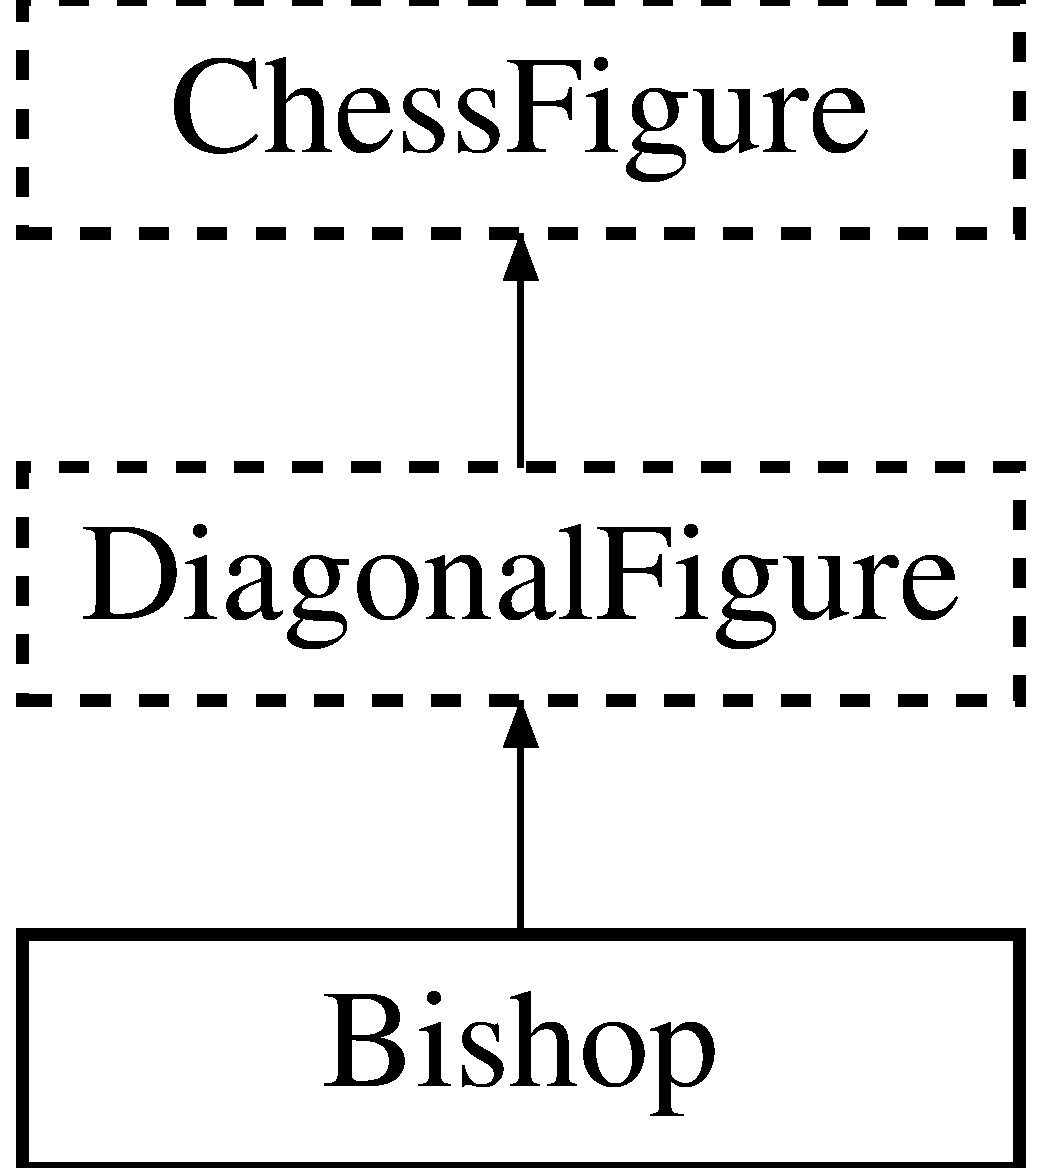
\includegraphics[height=3.000000cm]{classBishop}
\end{center}
\end{figure}
\subsection*{Public Member Functions}
\begin{DoxyCompactItemize}
\item 
\mbox{\Hypertarget{classBishop_a8e41c7d03936f10f1d7f78bb9b3a8b34}\label{classBishop_a8e41c7d03936f10f1d7f78bb9b3a8b34}} 
{\bfseries Bishop} (\mbox{\hyperlink{classChessFigure_a62f54318c1f28a08e6a6a2707f697a1d}{Team}} \mbox{\hyperlink{classChessFigure_ac7d0751a28c94d49927b9524390d1261}{team}})
\item 
\mbox{\Hypertarget{classBishop_a7255af36858df3d5349a9ab815afa9a7}\label{classBishop_a7255af36858df3d5349a9ab815afa9a7}} 
int \mbox{\hyperlink{classBishop_a7255af36858df3d5349a9ab815afa9a7}{get\+Value}} ()
\begin{DoxyCompactList}\small\item\em A getter function for the value of the figure (an AI can use it for weighting the figures) \end{DoxyCompactList}\item 
\mbox{\Hypertarget{classBishop_af2345c750c316768d046b064e6328b40}\label{classBishop_af2345c750c316768d046b064e6328b40}} 
std\+::string \mbox{\hyperlink{classBishop_af2345c750c316768d046b064e6328b40}{get\+Path}} ()
\begin{DoxyCompactList}\small\item\em The path to the image file of the figure. \end{DoxyCompactList}\item 
std\+::set$<$ \mbox{\hyperlink{classChessTile}{Chess\+Tile}} $\ast$ $>$ \mbox{\hyperlink{classBishop_a5da898db86a3025a5064d2d6ea2f1148}{get\+Step\+Options}} (\mbox{\hyperlink{classChessBoard}{Chess\+Board}} \&)
\begin{DoxyCompactList}\small\item\em A function that returns the available stepping options for the figure. \end{DoxyCompactList}\end{DoxyCompactItemize}
\subsection*{Additional Inherited Members}


\subsection{Member Function Documentation}
\mbox{\Hypertarget{classBishop_a5da898db86a3025a5064d2d6ea2f1148}\label{classBishop_a5da898db86a3025a5064d2d6ea2f1148}} 
\index{Bishop@{Bishop}!get\+Step\+Options@{get\+Step\+Options}}
\index{get\+Step\+Options@{get\+Step\+Options}!Bishop@{Bishop}}
\subsubsection{\texorpdfstring{get\+Step\+Options()}{getStepOptions()}}
{\footnotesize\ttfamily std\+::set$<$ \mbox{\hyperlink{classChessTile}{Chess\+Tile}} $\ast$ $>$ Bishop\+::get\+Step\+Options (\begin{DoxyParamCaption}\item[{\mbox{\hyperlink{classChessBoard}{Chess\+Board}} \&}]{board }\end{DoxyParamCaption})\hspace{0.3cm}{\ttfamily [virtual]}}



A function that returns the available stepping options for the figure. 


\begin{DoxyParams}{Parameters}
{\em board} & The \mbox{\hyperlink{classChessBoard}{Chess\+Board}} that the figure is placed on \\
\hline
\end{DoxyParams}


Implements \mbox{\hyperlink{classChessFigure_ae78d52e35c4ea926f492d211c69758bd}{Chess\+Figure}}.



The documentation for this class was generated from the following files\+:\begin{DoxyCompactItemize}
\item 
src/Chess\+Figures.\+h\item 
src/Chess\+Figures.\+cpp\end{DoxyCompactItemize}

\hypertarget{classChessBoard}{}\section{Chess\+Board Class Reference}
\label{classChessBoard}\index{Chess\+Board@{Chess\+Board}}
Inheritance diagram for Chess\+Board\+:\begin{figure}[H]
\begin{center}
\leavevmode
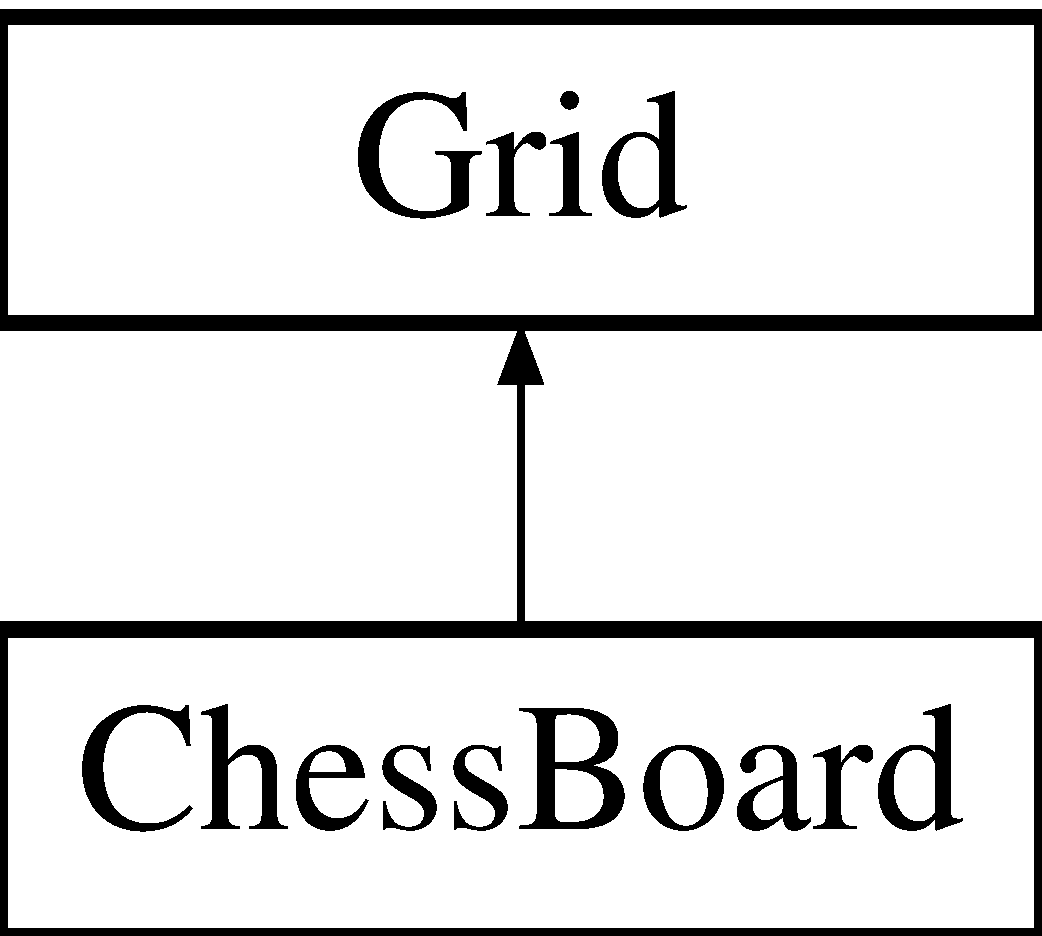
\includegraphics[height=2.000000cm]{classChessBoard}
\end{center}
\end{figure}
\subsection*{Public Member Functions}
\begin{DoxyCompactItemize}
\item 
\mbox{\Hypertarget{classChessBoard_ab905b19c4a54f58d3e9490ae058d50f3}\label{classChessBoard_ab905b19c4a54f58d3e9490ae058d50f3}} 
{\bfseries Chess\+Board} (int=8, int=8)
\item 
\mbox{\Hypertarget{classChessBoard_aa52c65d2811e1b16f645968c7376e490}\label{classChessBoard_aa52c65d2811e1b16f645968c7376e490}} 
{\bfseries Chess\+Board} (\mbox{\hyperlink{classChessBoard}{Chess\+Board}} \&)=delete
\item 
\mbox{\Hypertarget{classChessBoard_a5fef5d9dd63b08d21926fa357633d7a3}\label{classChessBoard_a5fef5d9dd63b08d21926fa357633d7a3}} 
\mbox{\hyperlink{classChessTile}{Chess\+Tile}} $\ast$$\ast$\& {\bfseries operator\mbox{[}$\,$\mbox{]}} (int)
\item 
\mbox{\Hypertarget{classChessBoard_a7f2b454b63cad50b551a42995fe20b92}\label{classChessBoard_a7f2b454b63cad50b551a42995fe20b92}} 
void {\bfseries fill\+With\+Tiles} ()
\item 
\mbox{\Hypertarget{classChessBoard_a104b758d5c28f2b31e12d34b467c37f5}\label{classChessBoard_a104b758d5c28f2b31e12d34b467c37f5}} 
void {\bfseries fill\+Board} ()
\item 
\mbox{\Hypertarget{classChessBoard_a91e32cb7b5139c304d552a4148030033}\label{classChessBoard_a91e32cb7b5139c304d552a4148030033}} 
void {\bfseries button\+Clicked} (\mbox{\hyperlink{classChessTile}{Chess\+Tile}} $\ast$)
\item 
\mbox{\Hypertarget{classChessBoard_acc60486a0fafa95c85263e15e6b7f6ab}\label{classChessBoard_acc60486a0fafa95c85263e15e6b7f6ab}} 
int {\bfseries getN} ()
\item 
\mbox{\Hypertarget{classChessBoard_a490cb74dc406003683738ab23372e66e}\label{classChessBoard_a490cb74dc406003683738ab23372e66e}} 
int {\bfseries getM} ()
\end{DoxyCompactItemize}


The documentation for this class was generated from the following files\+:\begin{DoxyCompactItemize}
\item 
src/Chess\+Board.\+h\item 
src/Chess\+Board.\+cpp\end{DoxyCompactItemize}

\hypertarget{classChessFigure}{}\section{Chess\+Figure Class Reference}
\label{classChessFigure}\index{Chess\+Figure@{Chess\+Figure}}


An abstract class that represents the chessfigures.  




{\ttfamily \#include $<$Chess\+Figures.\+h$>$}

Inheritance diagram for Chess\+Figure\+:\begin{figure}[H]
\begin{center}
\leavevmode
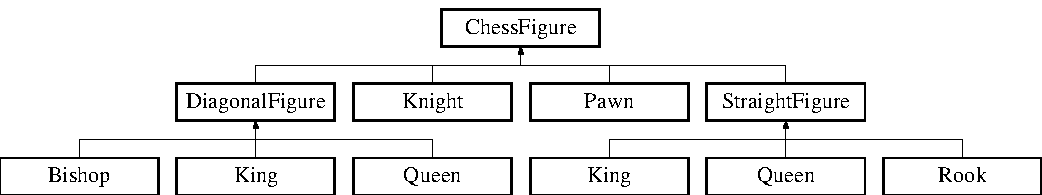
\includegraphics[height=2.616822cm]{classChessFigure}
\end{center}
\end{figure}
\subsection*{Public Types}
\begin{DoxyCompactItemize}
\item 
\mbox{\Hypertarget{classChessFigure_a62f54318c1f28a08e6a6a2707f697a1d}\label{classChessFigure_a62f54318c1f28a08e6a6a2707f697a1d}} 
enum \mbox{\hyperlink{classChessFigure_a62f54318c1f28a08e6a6a2707f697a1d}{Team}} \{ {\bfseries W\+H\+I\+TE}, 
{\bfseries B\+L\+A\+CK}
 \}
\begin{DoxyCompactList}\small\item\em An enum that can represent the team of the figure (white/black) \end{DoxyCompactList}\end{DoxyCompactItemize}
\subsection*{Public Member Functions}
\begin{DoxyCompactItemize}
\item 
\mbox{\hyperlink{classChessFigure_a09347f3c6276fc99ec111e44d2095c88}{Chess\+Figure}} (\mbox{\hyperlink{classChessFigure_a62f54318c1f28a08e6a6a2707f697a1d}{Team}} \mbox{\hyperlink{classChessFigure_ac7d0751a28c94d49927b9524390d1261}{team}})
\begin{DoxyCompactList}\small\item\em A contructor that expects the team of the figure. \end{DoxyCompactList}\item 
\mbox{\Hypertarget{classChessFigure_a7680676e4b3089ee8c0b1a424c71ec35}\label{classChessFigure_a7680676e4b3089ee8c0b1a424c71ec35}} 
\mbox{\hyperlink{classChessFigure_a62f54318c1f28a08e6a6a2707f697a1d}{Team}} \mbox{\hyperlink{classChessFigure_a7680676e4b3089ee8c0b1a424c71ec35}{get\+Team}} ()
\begin{DoxyCompactList}\small\item\em A getter function for the team variable. \end{DoxyCompactList}\item 
\mbox{\Hypertarget{classChessFigure_a5024e1c8c06e0e769c119de2d63a5ab8}\label{classChessFigure_a5024e1c8c06e0e769c119de2d63a5ab8}} 
virtual int \mbox{\hyperlink{classChessFigure_a5024e1c8c06e0e769c119de2d63a5ab8}{get\+Value}} ()=0
\begin{DoxyCompactList}\small\item\em A getter function for the value of the figure (an AI can use it for weighting the figures) \end{DoxyCompactList}\item 
\mbox{\Hypertarget{classChessFigure_aa8eef5ce3812121d417499cc7ab8b0b1}\label{classChessFigure_aa8eef5ce3812121d417499cc7ab8b0b1}} 
virtual std\+::string \mbox{\hyperlink{classChessFigure_aa8eef5ce3812121d417499cc7ab8b0b1}{get\+Path}} ()=0
\begin{DoxyCompactList}\small\item\em The path to the image file of the figure. \end{DoxyCompactList}\item 
virtual std\+::set$<$ \mbox{\hyperlink{classChessTile}{Chess\+Tile}} $\ast$ $>$ \mbox{\hyperlink{classChessFigure_ae78d52e35c4ea926f492d211c69758bd}{get\+Step\+Options}} (\mbox{\hyperlink{classChessBoard}{Chess\+Board}} \&board)=0
\begin{DoxyCompactList}\small\item\em A function that returns the available stepping options for the figure. \end{DoxyCompactList}\end{DoxyCompactItemize}
\subsection*{Protected Attributes}
\begin{DoxyCompactItemize}
\item 
\mbox{\Hypertarget{classChessFigure_ac7d0751a28c94d49927b9524390d1261}\label{classChessFigure_ac7d0751a28c94d49927b9524390d1261}} 
\mbox{\hyperlink{classChessFigure_a62f54318c1f28a08e6a6a2707f697a1d}{Team}} \mbox{\hyperlink{classChessFigure_ac7d0751a28c94d49927b9524390d1261}{team}}
\begin{DoxyCompactList}\small\item\em The figure\textquotesingle{}s team. \end{DoxyCompactList}\end{DoxyCompactItemize}


\subsection{Detailed Description}
An abstract class that represents the chessfigures. 

\subsection{Constructor \& Destructor Documentation}
\mbox{\Hypertarget{classChessFigure_a09347f3c6276fc99ec111e44d2095c88}\label{classChessFigure_a09347f3c6276fc99ec111e44d2095c88}} 
\index{Chess\+Figure@{Chess\+Figure}!Chess\+Figure@{Chess\+Figure}}
\index{Chess\+Figure@{Chess\+Figure}!Chess\+Figure@{Chess\+Figure}}
\subsubsection{\texorpdfstring{Chess\+Figure()}{ChessFigure()}}
{\footnotesize\ttfamily Chess\+Figure\+::\+Chess\+Figure (\begin{DoxyParamCaption}\item[{\mbox{\hyperlink{classChessFigure_a62f54318c1f28a08e6a6a2707f697a1d}{Team}}}]{team }\end{DoxyParamCaption})}



A contructor that expects the team of the figure. 


\begin{DoxyParams}{Parameters}
{\em team} & the team of the figure \\
\hline
\end{DoxyParams}


\subsection{Member Function Documentation}
\mbox{\Hypertarget{classChessFigure_ae78d52e35c4ea926f492d211c69758bd}\label{classChessFigure_ae78d52e35c4ea926f492d211c69758bd}} 
\index{Chess\+Figure@{Chess\+Figure}!get\+Step\+Options@{get\+Step\+Options}}
\index{get\+Step\+Options@{get\+Step\+Options}!Chess\+Figure@{Chess\+Figure}}
\subsubsection{\texorpdfstring{get\+Step\+Options()}{getStepOptions()}}
{\footnotesize\ttfamily virtual std\+::set$<$\mbox{\hyperlink{classChessTile}{Chess\+Tile}} $\ast$$>$ Chess\+Figure\+::get\+Step\+Options (\begin{DoxyParamCaption}\item[{\mbox{\hyperlink{classChessBoard}{Chess\+Board}} \&}]{board }\end{DoxyParamCaption})\hspace{0.3cm}{\ttfamily [pure virtual]}}



A function that returns the available stepping options for the figure. 


\begin{DoxyParams}{Parameters}
{\em board} & The \mbox{\hyperlink{classChessBoard}{Chess\+Board}} that the figure is placed on \\
\hline
\end{DoxyParams}


Implemented in \mbox{\hyperlink{classKnight_abb638cd75748653ec35365a77d528c42}{Knight}}, \mbox{\hyperlink{classRook_a466f48269ca58857c2a1ab1ab92c91f8}{Rook}}, \mbox{\hyperlink{classBishop_a5da898db86a3025a5064d2d6ea2f1148}{Bishop}}, \mbox{\hyperlink{classPawn_aa05272b9dcf50914ca51c5be1fe2d014}{Pawn}}, \mbox{\hyperlink{classQueen_a0fe4b1feaa74c1b2879ce991771054b0}{Queen}}, and \mbox{\hyperlink{classKing_a69703f80ac8c30335e4d745ee11518d7}{King}}.



The documentation for this class was generated from the following files\+:\begin{DoxyCompactItemize}
\item 
src/Chess\+Figures.\+h\item 
src/Chess\+Figures.\+cpp\end{DoxyCompactItemize}

\hypertarget{classChessTile}{}\section{Chess\+Tile Class Reference}
\label{classChessTile}\index{Chess\+Tile@{Chess\+Tile}}


A class that represents a tile of the board.  




{\ttfamily \#include $<$Chess\+Tile.\+h$>$}

Inheritance diagram for Chess\+Tile\+:\begin{figure}[H]
\begin{center}
\leavevmode
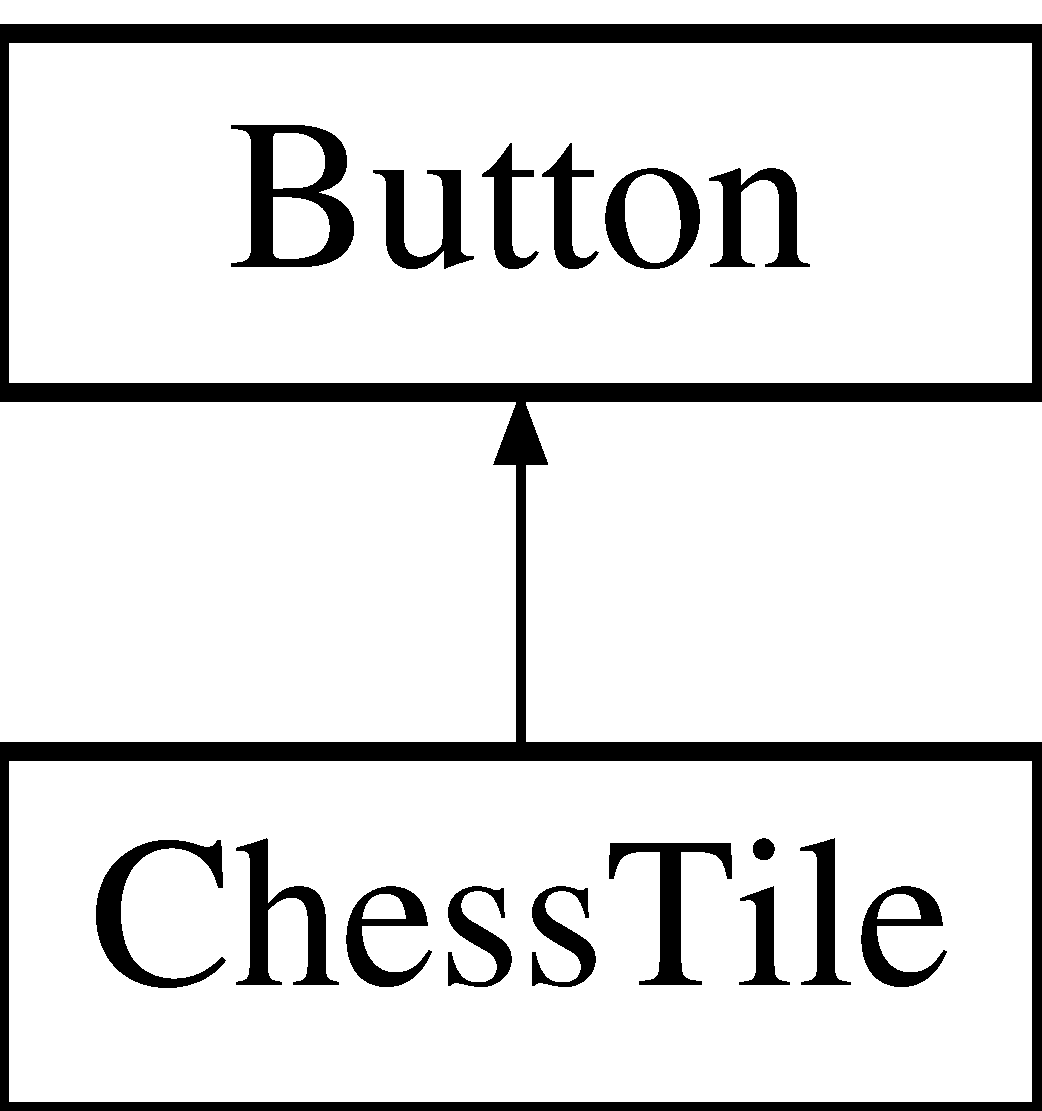
\includegraphics[height=2.000000cm]{classChessTile}
\end{center}
\end{figure}
\subsection*{Public Types}
\begin{DoxyCompactItemize}
\item 
\mbox{\Hypertarget{classChessTile_a9c573776c908586046e63facd4756e4d}\label{classChessTile_a9c573776c908586046e63facd4756e4d}} 
enum \mbox{\hyperlink{classChessTile_a9c573776c908586046e63facd4756e4d}{Colour}} \{ {\bfseries W\+H\+I\+TE}, 
{\bfseries B\+L\+A\+CK}
 \}
\begin{DoxyCompactList}\small\item\em An enum that represents the background colour of the tile. \end{DoxyCompactList}\end{DoxyCompactItemize}
\subsection*{Public Member Functions}
\begin{DoxyCompactItemize}
\item 
\mbox{\Hypertarget{classChessTile_a73d03ca0ed979d33e05316b9b14c20d2}\label{classChessTile_a73d03ca0ed979d33e05316b9b14c20d2}} 
\mbox{\hyperlink{classChessTile_a73d03ca0ed979d33e05316b9b14c20d2}{Chess\+Tile}} (\mbox{\hyperlink{classChessTile_a9c573776c908586046e63facd4756e4d}{Colour}})
\begin{DoxyCompactList}\small\item\em A constructor expecting a Colour. \end{DoxyCompactList}\item 
\mbox{\Hypertarget{classChessTile_a20bec4843dae5df211f99bc26b18c9b5}\label{classChessTile_a20bec4843dae5df211f99bc26b18c9b5}} 
{\bfseries Chess\+Tile} (\mbox{\hyperlink{classChessTile}{Chess\+Tile}} \&)=delete
\item 
\mbox{\Hypertarget{classChessTile_ae9dc270be7b2b2b7427eb7bc5e9b2842}\label{classChessTile_ae9dc270be7b2b2b7427eb7bc5e9b2842}} 
\mbox{\hyperlink{classChessTile}{Chess\+Tile}} \& \mbox{\hyperlink{classChessTile_ae9dc270be7b2b2b7427eb7bc5e9b2842}{operator=}} (\mbox{\hyperlink{classChessFigure}{Chess\+Figure}} $\ast$)
\begin{DoxyCompactList}\small\item\em The assign operator can be used to set the figure. \end{DoxyCompactList}\item 
\mbox{\Hypertarget{classChessTile_a310a1691be6e8e58f452ec817ab3db2f}\label{classChessTile_a310a1691be6e8e58f452ec817ab3db2f}} 
void \mbox{\hyperlink{classChessTile_a310a1691be6e8e58f452ec817ab3db2f}{reset\+Colour}} ()
\begin{DoxyCompactList}\small\item\em Sets the colour of the tile to the colour found in the colour variable. \end{DoxyCompactList}\item 
\mbox{\Hypertarget{classChessTile_af88f05cd0b3ea319cd11a78aec92499f}\label{classChessTile_af88f05cd0b3ea319cd11a78aec92499f}} 
\mbox{\hyperlink{classChessTile_a9c573776c908586046e63facd4756e4d}{Colour}} \mbox{\hyperlink{classChessTile_af88f05cd0b3ea319cd11a78aec92499f}{get\+Colour}} ()
\begin{DoxyCompactList}\small\item\em Returns the background colour of the board (B\+L\+A\+C\+K/\+W\+H\+I\+TE) \end{DoxyCompactList}\item 
\mbox{\Hypertarget{classChessTile_a31724ea2e6019fb367b8b2e8812d8fa6}\label{classChessTile_a31724ea2e6019fb367b8b2e8812d8fa6}} 
void \mbox{\hyperlink{classChessTile_a31724ea2e6019fb367b8b2e8812d8fa6}{set\+Figure}} (\mbox{\hyperlink{classChessFigure}{Chess\+Figure}} $\ast$)
\begin{DoxyCompactList}\small\item\em Sets the figure. \end{DoxyCompactList}\item 
\mbox{\Hypertarget{classChessTile_a3e6e2cb3d4582c05b48804105beeafb6}\label{classChessTile_a3e6e2cb3d4582c05b48804105beeafb6}} 
void \mbox{\hyperlink{classChessTile_a3e6e2cb3d4582c05b48804105beeafb6}{remove\+Figure}} ()
\begin{DoxyCompactList}\small\item\em Removes the figure. \end{DoxyCompactList}\item 
\mbox{\Hypertarget{classChessTile_a7aecc8930e76dc4ea934abe16dc68dcb}\label{classChessTile_a7aecc8930e76dc4ea934abe16dc68dcb}} 
\mbox{\hyperlink{classChessFigure}{Chess\+Figure}} $\ast$ \mbox{\hyperlink{classChessTile_a7aecc8930e76dc4ea934abe16dc68dcb}{get\+Figure}} ()
\begin{DoxyCompactList}\small\item\em Returns the figure. \end{DoxyCompactList}\end{DoxyCompactItemize}


\subsection{Detailed Description}
A class that represents a tile of the board. 

The documentation for this class was generated from the following files\+:\begin{DoxyCompactItemize}
\item 
src/Chess\+Tile.\+h\item 
src/Chess\+Tile.\+cpp\end{DoxyCompactItemize}

\hypertarget{classDiagonalFigure}{}\section{Diagonal\+Figure Class Reference}
\label{classDiagonalFigure}\index{Diagonal\+Figure@{Diagonal\+Figure}}
Inheritance diagram for Diagonal\+Figure\+:\begin{figure}[H]
\begin{center}
\leavevmode
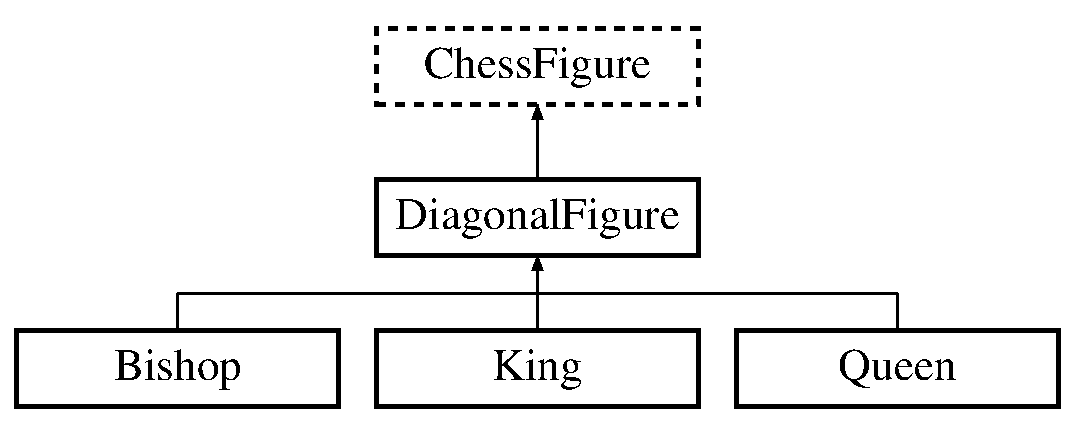
\includegraphics[height=3.000000cm]{classDiagonalFigure}
\end{center}
\end{figure}
\subsection*{Public Member Functions}
\begin{DoxyCompactItemize}
\item 
\mbox{\Hypertarget{classDiagonalFigure_a6fee4161066f638dda40b16d0096487d}\label{classDiagonalFigure_a6fee4161066f638dda40b16d0096487d}} 
virtual int \mbox{\hyperlink{classDiagonalFigure_a6fee4161066f638dda40b16d0096487d}{get\+Value}} ()=0
\begin{DoxyCompactList}\small\item\em A getter function for the value of the figure (an AI can use it for weighting the figures) \end{DoxyCompactList}\item 
\mbox{\Hypertarget{classDiagonalFigure_a95b5c28c86337d7d6b034aadd09c9d2b}\label{classDiagonalFigure_a95b5c28c86337d7d6b034aadd09c9d2b}} 
std\+::set$<$ \mbox{\hyperlink{classChessTile}{Chess\+Tile}} $\ast$ $>$ {\bfseries get\+Diagonal\+Stepping\+Options} (\mbox{\hyperlink{classChessBoard}{Chess\+Board}} \&, int, int, int)
\end{DoxyCompactItemize}
\subsection*{Additional Inherited Members}


The documentation for this class was generated from the following files\+:\begin{DoxyCompactItemize}
\item 
src/Chess\+Figures.\+h\item 
src/Chess\+Figures.\+cpp\end{DoxyCompactItemize}

\hypertarget{classKing}{}\section{King Class Reference}
\label{classKing}\index{King@{King}}


A class that represents king figures.  




{\ttfamily \#include $<$Chess\+Figures.\+h$>$}

Inheritance diagram for King\+:\begin{figure}[H]
\begin{center}
\leavevmode
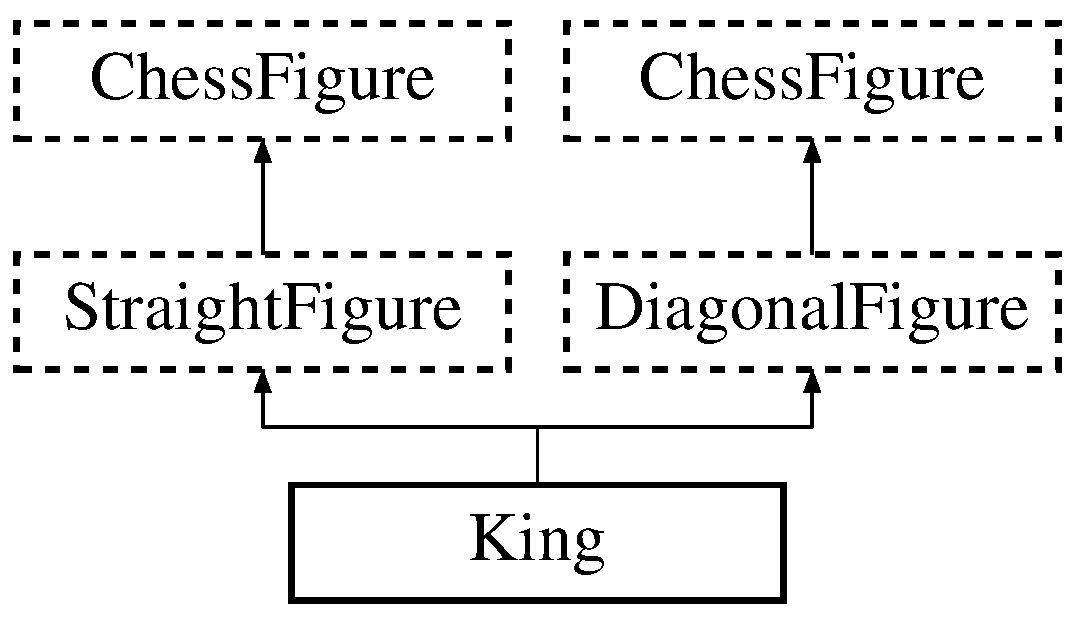
\includegraphics[height=3.000000cm]{classKing}
\end{center}
\end{figure}
\subsection*{Public Member Functions}
\begin{DoxyCompactItemize}
\item 
\mbox{\Hypertarget{classKing_a3e945491cb38d473fcd809c11c15129e}\label{classKing_a3e945491cb38d473fcd809c11c15129e}} 
\mbox{\hyperlink{classKing_a3e945491cb38d473fcd809c11c15129e}{King}} (\mbox{\hyperlink{classChessFigure_a62f54318c1f28a08e6a6a2707f697a1d}{Team}} \mbox{\hyperlink{classChessFigure_ac7d0751a28c94d49927b9524390d1261}{team}})
\begin{DoxyCompactList}\small\item\em A constructor expecting a Team. \end{DoxyCompactList}\item 
\mbox{\Hypertarget{classKing_a4778898c5534c04dd93194d22ef317c3}\label{classKing_a4778898c5534c04dd93194d22ef317c3}} 
int \mbox{\hyperlink{classKing_a4778898c5534c04dd93194d22ef317c3}{get\+Value}} ()
\begin{DoxyCompactList}\small\item\em A getter function for the value of the figure (an AI can use it for weighting the figures) \end{DoxyCompactList}\item 
\mbox{\Hypertarget{classKing_a29a27a0f1280bb352d601d0aeeea13f1}\label{classKing_a29a27a0f1280bb352d601d0aeeea13f1}} 
std\+::string \mbox{\hyperlink{classKing_a29a27a0f1280bb352d601d0aeeea13f1}{get\+Path}} ()
\begin{DoxyCompactList}\small\item\em The path to the image file of the figure. \end{DoxyCompactList}\item 
std\+::set$<$ \mbox{\hyperlink{classChessTile}{Chess\+Tile}} $\ast$ $>$ \mbox{\hyperlink{classKing_a69703f80ac8c30335e4d745ee11518d7}{get\+Step\+Options}} (\mbox{\hyperlink{classChessBoard}{Chess\+Board}} \&)
\begin{DoxyCompactList}\small\item\em A function that returns the available stepping options for the figure. \end{DoxyCompactList}\end{DoxyCompactItemize}
\subsection*{Additional Inherited Members}


\subsection{Detailed Description}
A class that represents king figures. 

\subsection{Member Function Documentation}
\mbox{\Hypertarget{classKing_a69703f80ac8c30335e4d745ee11518d7}\label{classKing_a69703f80ac8c30335e4d745ee11518d7}} 
\index{King@{King}!get\+Step\+Options@{get\+Step\+Options}}
\index{get\+Step\+Options@{get\+Step\+Options}!King@{King}}
\subsubsection{\texorpdfstring{get\+Step\+Options()}{getStepOptions()}}
{\footnotesize\ttfamily std\+::set$<$ \mbox{\hyperlink{classChessTile}{Chess\+Tile}} $\ast$ $>$ King\+::get\+Step\+Options (\begin{DoxyParamCaption}\item[{\mbox{\hyperlink{classChessBoard}{Chess\+Board}} \&}]{board }\end{DoxyParamCaption})\hspace{0.3cm}{\ttfamily [virtual]}}



A function that returns the available stepping options for the figure. 


\begin{DoxyParams}{Parameters}
{\em board} & The \mbox{\hyperlink{classChessBoard}{Chess\+Board}} that the figure is placed on \\
\hline
\end{DoxyParams}


Implements \mbox{\hyperlink{classChessFigure_ae78d52e35c4ea926f492d211c69758bd}{Chess\+Figure}}.



The documentation for this class was generated from the following files\+:\begin{DoxyCompactItemize}
\item 
src/Chess\+Figures.\+h\item 
src/Chess\+Figures.\+cpp\end{DoxyCompactItemize}

\hypertarget{classKnight}{}\section{Knight Class Reference}
\label{classKnight}\index{Knight@{Knight}}


A class that represents knight figures.  




{\ttfamily \#include $<$Chess\+Figures.\+h$>$}

Inheritance diagram for Knight\+:\begin{figure}[H]
\begin{center}
\leavevmode
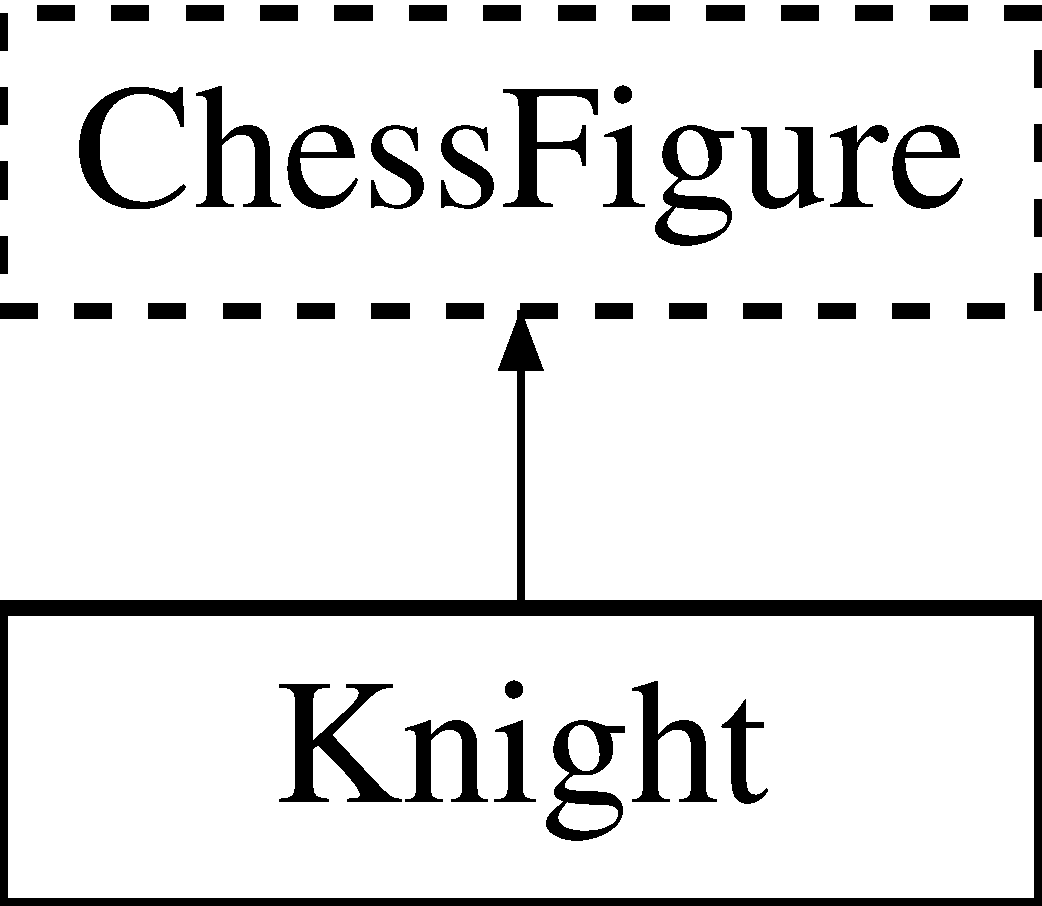
\includegraphics[height=2.000000cm]{classKnight}
\end{center}
\end{figure}
\subsection*{Public Member Functions}
\begin{DoxyCompactItemize}
\item 
\mbox{\Hypertarget{classKnight_aee4103f3beddb7aecb291f578c6a64e1}\label{classKnight_aee4103f3beddb7aecb291f578c6a64e1}} 
\mbox{\hyperlink{classKnight_aee4103f3beddb7aecb291f578c6a64e1}{Knight}} (\mbox{\hyperlink{classChessFigure_a62f54318c1f28a08e6a6a2707f697a1d}{Team}} \mbox{\hyperlink{classChessFigure_ac7d0751a28c94d49927b9524390d1261}{team}})
\begin{DoxyCompactList}\small\item\em A constructor expecting a Team. \end{DoxyCompactList}\item 
\mbox{\Hypertarget{classKnight_af0a9bd91ab46869e921b9cbf7a894e44}\label{classKnight_af0a9bd91ab46869e921b9cbf7a894e44}} 
int \mbox{\hyperlink{classKnight_af0a9bd91ab46869e921b9cbf7a894e44}{get\+Value}} ()
\begin{DoxyCompactList}\small\item\em A getter function for the value of the figure (an AI can use it for weighting the figures) \end{DoxyCompactList}\item 
\mbox{\Hypertarget{classKnight_a0df5d1725855c2bf6189258ff8f4e675}\label{classKnight_a0df5d1725855c2bf6189258ff8f4e675}} 
std\+::string \mbox{\hyperlink{classKnight_a0df5d1725855c2bf6189258ff8f4e675}{get\+Path}} ()
\begin{DoxyCompactList}\small\item\em The path to the image file of the figure. \end{DoxyCompactList}\item 
std\+::set$<$ \mbox{\hyperlink{classChessTile}{Chess\+Tile}} $\ast$ $>$ \mbox{\hyperlink{classKnight_abb638cd75748653ec35365a77d528c42}{get\+Step\+Options}} (\mbox{\hyperlink{classChessBoard}{Chess\+Board}} \&)
\begin{DoxyCompactList}\small\item\em A function that returns the available stepping options for the figure. \end{DoxyCompactList}\end{DoxyCompactItemize}
\subsection*{Additional Inherited Members}


\subsection{Detailed Description}
A class that represents knight figures. 

\subsection{Member Function Documentation}
\mbox{\Hypertarget{classKnight_abb638cd75748653ec35365a77d528c42}\label{classKnight_abb638cd75748653ec35365a77d528c42}} 
\index{Knight@{Knight}!get\+Step\+Options@{get\+Step\+Options}}
\index{get\+Step\+Options@{get\+Step\+Options}!Knight@{Knight}}
\subsubsection{\texorpdfstring{get\+Step\+Options()}{getStepOptions()}}
{\footnotesize\ttfamily std\+::set$<$ \mbox{\hyperlink{classChessTile}{Chess\+Tile}} $\ast$ $>$ Knight\+::get\+Step\+Options (\begin{DoxyParamCaption}\item[{\mbox{\hyperlink{classChessBoard}{Chess\+Board}} \&}]{board }\end{DoxyParamCaption})\hspace{0.3cm}{\ttfamily [virtual]}}



A function that returns the available stepping options for the figure. 


\begin{DoxyParams}{Parameters}
{\em board} & The \mbox{\hyperlink{classChessBoard}{Chess\+Board}} that the figure is placed on \\
\hline
\end{DoxyParams}


Implements \mbox{\hyperlink{classChessFigure_ae78d52e35c4ea926f492d211c69758bd}{Chess\+Figure}}.



The documentation for this class was generated from the following files\+:\begin{DoxyCompactItemize}
\item 
src/Chess\+Figures.\+h\item 
src/Chess\+Figures.\+cpp\end{DoxyCompactItemize}

\hypertarget{classPawn}{}\section{Pawn Class Reference}
\label{classPawn}\index{Pawn@{Pawn}}
Inheritance diagram for Pawn\+:\begin{figure}[H]
\begin{center}
\leavevmode
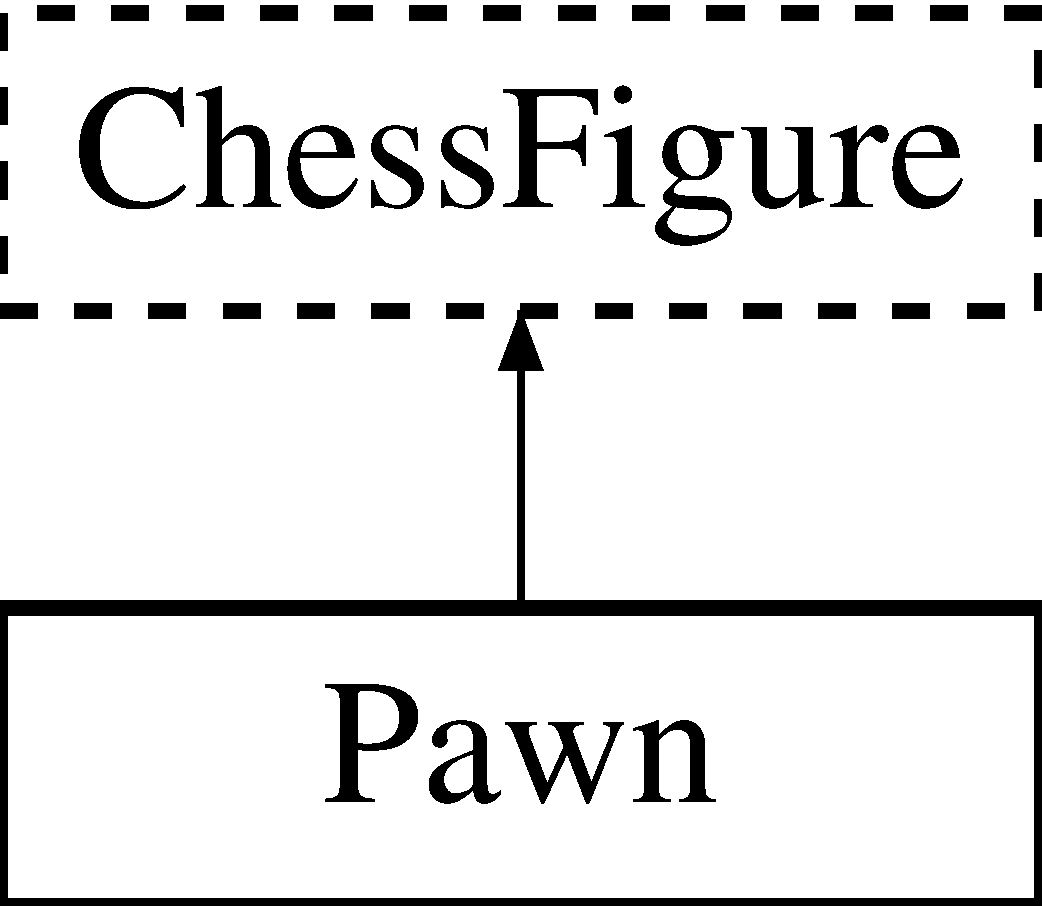
\includegraphics[height=2.000000cm]{classPawn}
\end{center}
\end{figure}
\subsection*{Public Member Functions}
\begin{DoxyCompactItemize}
\item 
\mbox{\Hypertarget{classPawn_ab800634302e5af17a3d37cfe23f4cf15}\label{classPawn_ab800634302e5af17a3d37cfe23f4cf15}} 
{\bfseries Pawn} (\mbox{\hyperlink{classChessFigure_a62f54318c1f28a08e6a6a2707f697a1d}{Team}} \mbox{\hyperlink{classChessFigure_ac7d0751a28c94d49927b9524390d1261}{team}})
\item 
\mbox{\Hypertarget{classPawn_ab8d4325ff14660b70455c7b7acee221c}\label{classPawn_ab8d4325ff14660b70455c7b7acee221c}} 
int \mbox{\hyperlink{classPawn_ab8d4325ff14660b70455c7b7acee221c}{get\+Value}} ()
\begin{DoxyCompactList}\small\item\em A getter function for the value of the figure (an AI can use it for weighting the figures) \end{DoxyCompactList}\item 
\mbox{\Hypertarget{classPawn_a72fd4d337ecea0e41f2ffb1933643269}\label{classPawn_a72fd4d337ecea0e41f2ffb1933643269}} 
std\+::string \mbox{\hyperlink{classPawn_a72fd4d337ecea0e41f2ffb1933643269}{get\+Path}} ()
\begin{DoxyCompactList}\small\item\em The path to the image file of the figure. \end{DoxyCompactList}\item 
std\+::set$<$ \mbox{\hyperlink{classChessTile}{Chess\+Tile}} $\ast$ $>$ \mbox{\hyperlink{classPawn_aa05272b9dcf50914ca51c5be1fe2d014}{get\+Step\+Options}} (\mbox{\hyperlink{classChessBoard}{Chess\+Board}} \&)
\begin{DoxyCompactList}\small\item\em A function that returns the available stepping options for the figure. \end{DoxyCompactList}\end{DoxyCompactItemize}
\subsection*{Additional Inherited Members}


\subsection{Member Function Documentation}
\mbox{\Hypertarget{classPawn_aa05272b9dcf50914ca51c5be1fe2d014}\label{classPawn_aa05272b9dcf50914ca51c5be1fe2d014}} 
\index{Pawn@{Pawn}!get\+Step\+Options@{get\+Step\+Options}}
\index{get\+Step\+Options@{get\+Step\+Options}!Pawn@{Pawn}}
\subsubsection{\texorpdfstring{get\+Step\+Options()}{getStepOptions()}}
{\footnotesize\ttfamily std\+::set$<$ \mbox{\hyperlink{classChessTile}{Chess\+Tile}} $\ast$ $>$ Pawn\+::get\+Step\+Options (\begin{DoxyParamCaption}\item[{\mbox{\hyperlink{classChessBoard}{Chess\+Board}} \&}]{board }\end{DoxyParamCaption})\hspace{0.3cm}{\ttfamily [virtual]}}



A function that returns the available stepping options for the figure. 


\begin{DoxyParams}{Parameters}
{\em board} & The \mbox{\hyperlink{classChessBoard}{Chess\+Board}} that the figure is placed on \\
\hline
\end{DoxyParams}


Implements \mbox{\hyperlink{classChessFigure_ae78d52e35c4ea926f492d211c69758bd}{Chess\+Figure}}.



The documentation for this class was generated from the following files\+:\begin{DoxyCompactItemize}
\item 
src/Chess\+Figures.\+h\item 
src/Chess\+Figures.\+cpp\end{DoxyCompactItemize}

\hypertarget{classQueen}{}\section{Queen Class Reference}
\label{classQueen}\index{Queen@{Queen}}


A class that represents queen figures.  




{\ttfamily \#include $<$Chess\+Figures.\+h$>$}

Inheritance diagram for Queen\+:\begin{figure}[H]
\begin{center}
\leavevmode
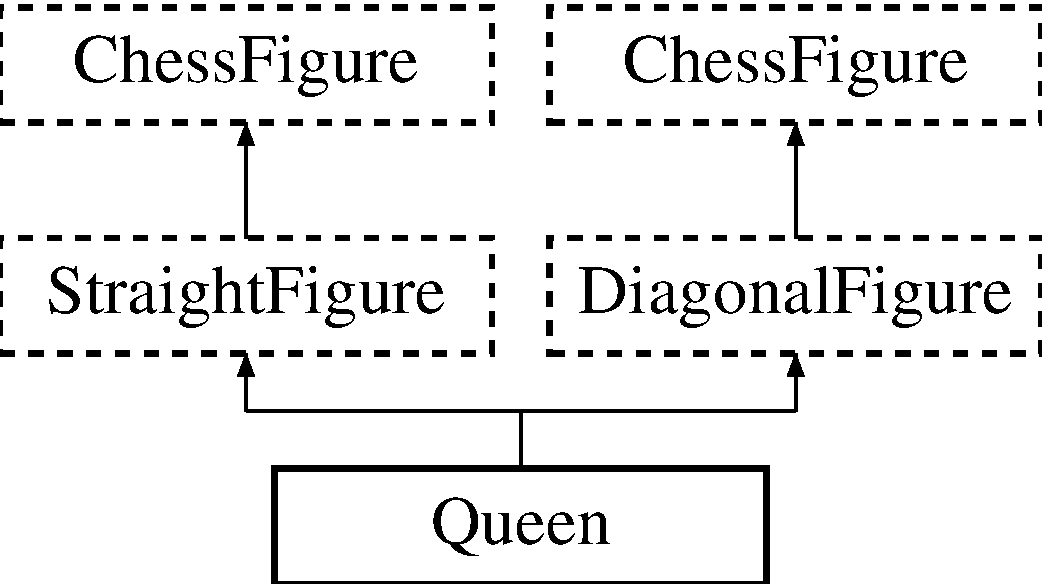
\includegraphics[height=3.000000cm]{classQueen}
\end{center}
\end{figure}
\subsection*{Public Member Functions}
\begin{DoxyCompactItemize}
\item 
\mbox{\Hypertarget{classQueen_aff683860a39f6b0e4c19505f8e28706f}\label{classQueen_aff683860a39f6b0e4c19505f8e28706f}} 
\mbox{\hyperlink{classQueen_aff683860a39f6b0e4c19505f8e28706f}{Queen}} (\mbox{\hyperlink{classChessFigure_a62f54318c1f28a08e6a6a2707f697a1d}{Team}} \mbox{\hyperlink{classChessFigure_ac7d0751a28c94d49927b9524390d1261}{team}})
\begin{DoxyCompactList}\small\item\em A constructor expecting a Team. \end{DoxyCompactList}\item 
\mbox{\Hypertarget{classQueen_a88e9312353dc2443ad658de7495b86b8}\label{classQueen_a88e9312353dc2443ad658de7495b86b8}} 
int \mbox{\hyperlink{classQueen_a88e9312353dc2443ad658de7495b86b8}{get\+Value}} ()
\begin{DoxyCompactList}\small\item\em A getter function for the value of the figure (an AI can use it for weighting the figures) \end{DoxyCompactList}\item 
\mbox{\Hypertarget{classQueen_a0f41324a91413c415b1cf19fb52447c4}\label{classQueen_a0f41324a91413c415b1cf19fb52447c4}} 
std\+::string \mbox{\hyperlink{classQueen_a0f41324a91413c415b1cf19fb52447c4}{get\+Path}} ()
\begin{DoxyCompactList}\small\item\em The path to the image file of the figure. \end{DoxyCompactList}\item 
std\+::set$<$ \mbox{\hyperlink{classChessTile}{Chess\+Tile}} $\ast$ $>$ \mbox{\hyperlink{classQueen_a0fe4b1feaa74c1b2879ce991771054b0}{get\+Step\+Options}} (\mbox{\hyperlink{classChessBoard}{Chess\+Board}} \&)
\begin{DoxyCompactList}\small\item\em A function that returns the available stepping options for the figure. \end{DoxyCompactList}\end{DoxyCompactItemize}
\subsection*{Additional Inherited Members}


\subsection{Detailed Description}
A class that represents queen figures. 

\subsection{Member Function Documentation}
\mbox{\Hypertarget{classQueen_a0fe4b1feaa74c1b2879ce991771054b0}\label{classQueen_a0fe4b1feaa74c1b2879ce991771054b0}} 
\index{Queen@{Queen}!get\+Step\+Options@{get\+Step\+Options}}
\index{get\+Step\+Options@{get\+Step\+Options}!Queen@{Queen}}
\subsubsection{\texorpdfstring{get\+Step\+Options()}{getStepOptions()}}
{\footnotesize\ttfamily std\+::set$<$ \mbox{\hyperlink{classChessTile}{Chess\+Tile}} $\ast$ $>$ Queen\+::get\+Step\+Options (\begin{DoxyParamCaption}\item[{\mbox{\hyperlink{classChessBoard}{Chess\+Board}} \&}]{board }\end{DoxyParamCaption})\hspace{0.3cm}{\ttfamily [virtual]}}



A function that returns the available stepping options for the figure. 


\begin{DoxyParams}{Parameters}
{\em board} & The \mbox{\hyperlink{classChessBoard}{Chess\+Board}} that the figure is placed on \\
\hline
\end{DoxyParams}


Implements \mbox{\hyperlink{classChessFigure_ae78d52e35c4ea926f492d211c69758bd}{Chess\+Figure}}.



The documentation for this class was generated from the following files\+:\begin{DoxyCompactItemize}
\item 
src/Chess\+Figures.\+h\item 
src/Chess\+Figures.\+cpp\end{DoxyCompactItemize}

\hypertarget{classRook}{}\section{Rook Class Reference}
\label{classRook}\index{Rook@{Rook}}


A class that represents bishop figures.  




{\ttfamily \#include $<$Chess\+Figures.\+h$>$}

Inheritance diagram for Rook\+:\begin{figure}[H]
\begin{center}
\leavevmode
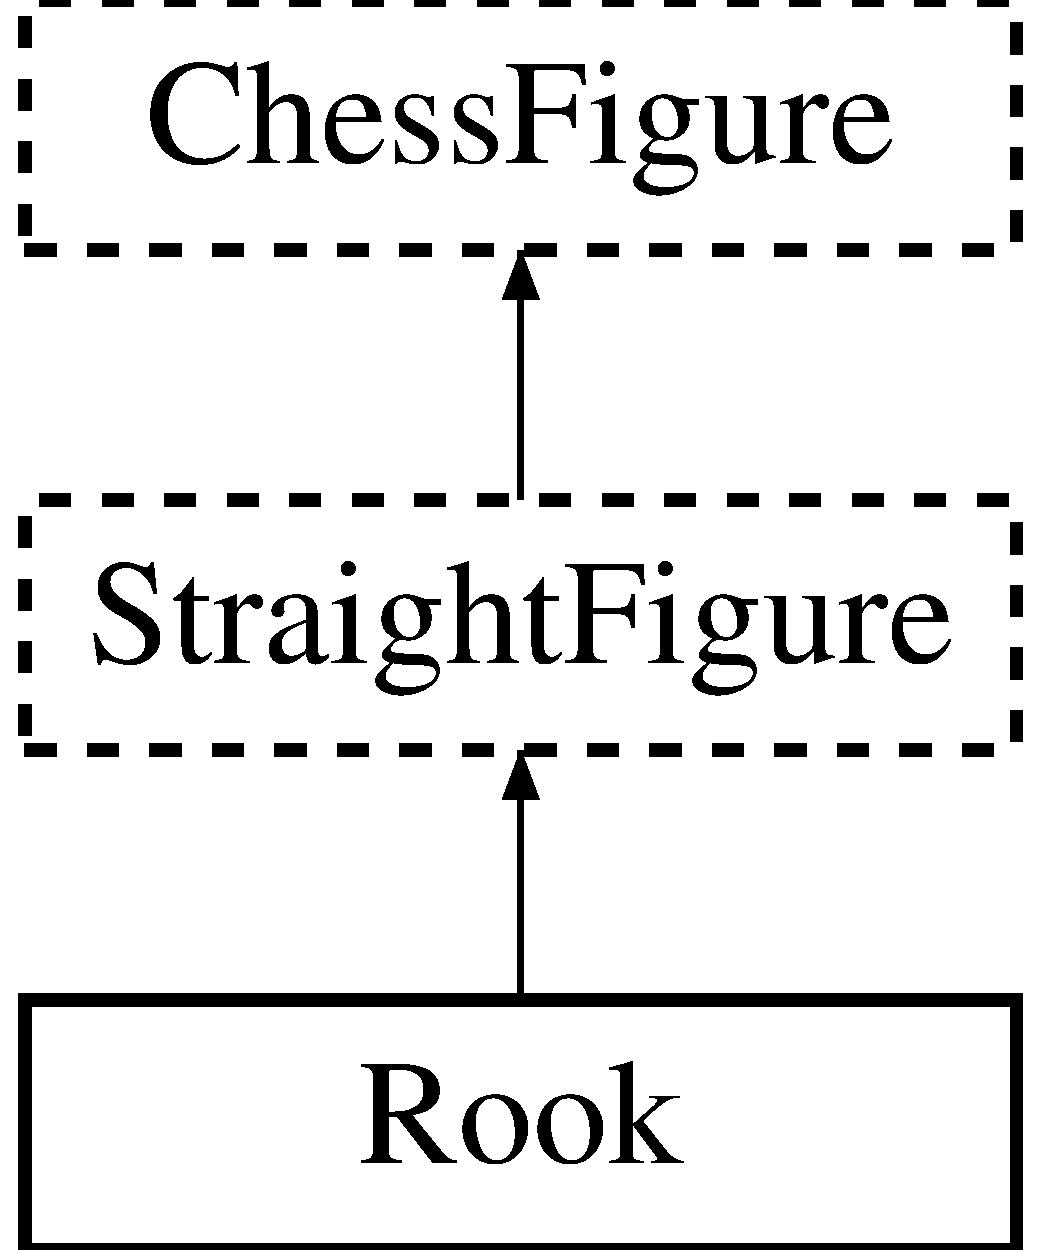
\includegraphics[height=3.000000cm]{classRook}
\end{center}
\end{figure}
\subsection*{Public Member Functions}
\begin{DoxyCompactItemize}
\item 
\mbox{\Hypertarget{classRook_abdf50f6076fa9c5fed408815b91a6e82}\label{classRook_abdf50f6076fa9c5fed408815b91a6e82}} 
\mbox{\hyperlink{classRook_abdf50f6076fa9c5fed408815b91a6e82}{Rook}} (\mbox{\hyperlink{classChessFigure_a62f54318c1f28a08e6a6a2707f697a1d}{Team}} \mbox{\hyperlink{classChessFigure_ac7d0751a28c94d49927b9524390d1261}{team}})
\begin{DoxyCompactList}\small\item\em A constructor expecting a Team. \end{DoxyCompactList}\item 
\mbox{\Hypertarget{classRook_ab3487b23185bb20b2b5306f9a5fe127b}\label{classRook_ab3487b23185bb20b2b5306f9a5fe127b}} 
int \mbox{\hyperlink{classRook_ab3487b23185bb20b2b5306f9a5fe127b}{get\+Value}} ()
\begin{DoxyCompactList}\small\item\em A getter function for the value of the figure (an AI can use it for weighting the figures) \end{DoxyCompactList}\item 
\mbox{\Hypertarget{classRook_a0cae7fbabe3169ec506fcd29ae396ba7}\label{classRook_a0cae7fbabe3169ec506fcd29ae396ba7}} 
std\+::string \mbox{\hyperlink{classRook_a0cae7fbabe3169ec506fcd29ae396ba7}{get\+Path}} ()
\begin{DoxyCompactList}\small\item\em The path to the image file of the figure. \end{DoxyCompactList}\item 
std\+::set$<$ \mbox{\hyperlink{classChessTile}{Chess\+Tile}} $\ast$ $>$ \mbox{\hyperlink{classRook_a466f48269ca58857c2a1ab1ab92c91f8}{get\+Step\+Options}} (\mbox{\hyperlink{classChessBoard}{Chess\+Board}} \&)
\begin{DoxyCompactList}\small\item\em A function that returns the available stepping options for the figure. \end{DoxyCompactList}\end{DoxyCompactItemize}
\subsection*{Additional Inherited Members}


\subsection{Detailed Description}
A class that represents bishop figures. 

\subsection{Member Function Documentation}
\mbox{\Hypertarget{classRook_a466f48269ca58857c2a1ab1ab92c91f8}\label{classRook_a466f48269ca58857c2a1ab1ab92c91f8}} 
\index{Rook@{Rook}!get\+Step\+Options@{get\+Step\+Options}}
\index{get\+Step\+Options@{get\+Step\+Options}!Rook@{Rook}}
\subsubsection{\texorpdfstring{get\+Step\+Options()}{getStepOptions()}}
{\footnotesize\ttfamily std\+::set$<$ \mbox{\hyperlink{classChessTile}{Chess\+Tile}} $\ast$ $>$ Rook\+::get\+Step\+Options (\begin{DoxyParamCaption}\item[{\mbox{\hyperlink{classChessBoard}{Chess\+Board}} \&}]{board }\end{DoxyParamCaption})\hspace{0.3cm}{\ttfamily [virtual]}}



A function that returns the available stepping options for the figure. 


\begin{DoxyParams}{Parameters}
{\em board} & The \mbox{\hyperlink{classChessBoard}{Chess\+Board}} that the figure is placed on \\
\hline
\end{DoxyParams}


Implements \mbox{\hyperlink{classChessFigure_ae78d52e35c4ea926f492d211c69758bd}{Chess\+Figure}}.



The documentation for this class was generated from the following files\+:\begin{DoxyCompactItemize}
\item 
src/Chess\+Figures.\+h\item 
src/Chess\+Figures.\+cpp\end{DoxyCompactItemize}

\hypertarget{classStraightFigure}{}\section{Straight\+Figure Class Reference}
\label{classStraightFigure}\index{Straight\+Figure@{Straight\+Figure}}


An.  




{\ttfamily \#include $<$Chess\+Figures.\+h$>$}

Inheritance diagram for Straight\+Figure\+:\begin{figure}[H]
\begin{center}
\leavevmode
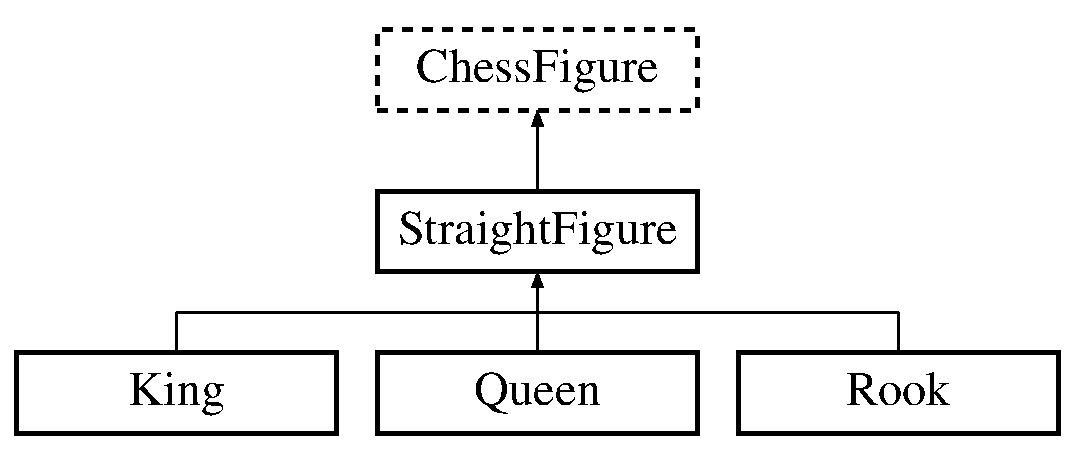
\includegraphics[height=3.000000cm]{classStraightFigure}
\end{center}
\end{figure}
\subsection*{Public Member Functions}
\begin{DoxyCompactItemize}
\item 
\mbox{\Hypertarget{classStraightFigure_a09d46ae2b3f043b9ac3e05ed6d95d420}\label{classStraightFigure_a09d46ae2b3f043b9ac3e05ed6d95d420}} 
virtual int \mbox{\hyperlink{classStraightFigure_a09d46ae2b3f043b9ac3e05ed6d95d420}{get\+Value}} ()=0
\begin{DoxyCompactList}\small\item\em A getter function for the value of the figure (an AI can use it for weighting the figures) \end{DoxyCompactList}\item 
\mbox{\Hypertarget{classStraightFigure_ac466b7394b41a10c582c9f363e907494}\label{classStraightFigure_ac466b7394b41a10c582c9f363e907494}} 
std\+::set$<$ \mbox{\hyperlink{classChessTile}{Chess\+Tile}} $\ast$ $>$ {\bfseries get\+Horizontal\+Stepping\+Options} (\mbox{\hyperlink{classChessBoard}{Chess\+Board}} \&, int, int, int)
\item 
\mbox{\Hypertarget{classStraightFigure_a9d0fd89679a129342adef0fd64c31dfa}\label{classStraightFigure_a9d0fd89679a129342adef0fd64c31dfa}} 
std\+::set$<$ \mbox{\hyperlink{classChessTile}{Chess\+Tile}} $\ast$ $>$ {\bfseries get\+Vertical\+Stepping\+Options} (\mbox{\hyperlink{classChessBoard}{Chess\+Board}} \&, int, int, int)
\end{DoxyCompactItemize}
\subsection*{Additional Inherited Members}


\subsection{Detailed Description}
An. 

The documentation for this class was generated from the following files\+:\begin{DoxyCompactItemize}
\item 
src/Chess\+Figures.\+h\item 
src/Chess\+Figures.\+cpp\end{DoxyCompactItemize}

\chapter{File Documentation}
\hypertarget{Chess_8cpp}{}\section{src/\+Chess.cpp File Reference}
\label{Chess_8cpp}\index{src/\+Chess.\+cpp@{src/\+Chess.\+cpp}}
{\ttfamily \#include $<$gtkmm.\+h$>$}\newline
{\ttfamily \#include $<$iostream$>$}\newline
{\ttfamily \#include \char`\"{}Chess\+Board.\+h\char`\"{}}\newline
{\ttfamily \#include \char`\"{}Chess\+Figures.\+h\char`\"{}}\newline
{\ttfamily \#include \char`\"{}Chess\+Tile.\+h\char`\"{}}\newline
{\ttfamily \#include $<$set$>$}\newline
\subsection*{Functions}
\begin{DoxyCompactItemize}
\item 
int \mbox{\hyperlink{Chess_8cpp_a0ddf1224851353fc92bfbff6f499fa97}{main}} (int argc, char $\ast$argv\mbox{[}$\,$\mbox{]})
\begin{DoxyCompactList}\small\item\em The main function of the program. \end{DoxyCompactList}\end{DoxyCompactItemize}


\subsection{Function Documentation}
\mbox{\Hypertarget{Chess_8cpp_a0ddf1224851353fc92bfbff6f499fa97}\label{Chess_8cpp_a0ddf1224851353fc92bfbff6f499fa97}} 
\index{Chess.\+cpp@{Chess.\+cpp}!main@{main}}
\index{main@{main}!Chess.\+cpp@{Chess.\+cpp}}
\subsubsection{\texorpdfstring{main()}{main()}}
{\footnotesize\ttfamily int main (\begin{DoxyParamCaption}\item[{int}]{argc,  }\item[{char $\ast$}]{argv\mbox{[}$\,$\mbox{]} }\end{DoxyParamCaption})}



The main function of the program. 

Creating a Gtk Application instance

Creating a window instance

Setting the size of the window

Creating a \mbox{\hyperlink{classChessBoard}{Chess\+Board}} instance

Filling the board with tiles

Filling the board with figures

Adding the board to the window

Asking the window to show all its children

Running the application 
%--- End generated contents ---

% Index
\backmatter
\newpage
\phantomsection
\clearemptydoublepage
\addcontentsline{toc}{chapter}{Index}
\printindex

\end{document}
